\documentclass{standalone}

\usepackage[OT1]{fontenc}
\renewcommand*\familydefault{\sfdefault}
\usepackage{helvet,sfmath}
\usepackage{siunitx}

\usepackage{tikz}
\usetikzlibrary{arrows,calc,patterns}
\usepackage{tikz,tkz-euclide}

\definecolor{BlueDefault}{rgb}{0.2,0.2,0.7}

\begin{document}

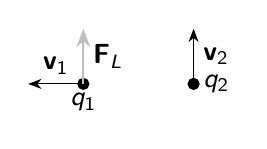
\begin{tikzpicture}[scale=0.7]
    \draw[-Stealth] (-1,0) to (-2,0);
    \draw[-Stealth] (1,0) to (1,1);
    \draw
    (-1.5,0) node[above]{\(\mathbf{v}_1\)}
    (1,0.5) node[right]{\(\mathbf{v}_2\)}
    ;
    \draw[fill = black] (-1,0) circle (0.1);
    \draw[fill = black] (1,0) circle (0.1);
    \draw
    (-1,0) node[below]{\(q_1\)}
    (1,0) node[right]{\(q_2\)}
    ;
    \draw[thick, lightgray, -Stealth] (-1,0) to (-1,1);
    \draw (-1,0.5) node[right]{\(\mathbf{F}_L\)};
\end{tikzpicture}

\end{document}